\part{Quinto semestre}
\chapterimage{5.pdf}
\chapter{Cálculo Diferencial}

\section{Razones de cambio} % 3 clases
\subsection{Introducción}
\begin{definition}[Razón de cambio]
    La razón de cambio de una función \( f(x) \) en un intervalo es una medida de cómo cambia el valor de \( f(x) \) con respecto al cambio en \( x \) en ese intervalo. Matemáticamente, se define como la derivada de \( f(x) \) en un punto \( x \), que es la pendiente de la línea tangente a la curva en ese punto
\end{definition}
La razón de cambio promedio de \( f(x) \) entre dos puntos \( x_1 \) y \( x_2 \) se define como:
\[
\text{Razón de cambio promedio} = \frac{f(x_2) - f(x_1)}{x_2 - x_1}
\]

La razón de cambio instantánea en un punto \( x \) es la derivada de \( f(x) \) en ese punto, que se denota por \( f'(x) \) o \( \frac{d}{dx} f(x) \):
\[
\text{Razón de cambio instantánea} = f'(x)
\]

\begin{example}
    
\textbf{Problema:} Consideremos la función \( f(x) = x^2 \). Queremos calcular la razón de cambio promedio entre \( x = 1 \) y \( x = 3 \) y la razón de cambio instantánea en \( x = 2 \).

\textbf{Solución:}

\begin{enumerate}
    \item  \textbf{Razón de cambio promedio:}
    \[
    \frac{f(3) - f(1)}{3 - 1} = \frac{3^2 - 1^2}{3 - 1} = \frac{9 - 1}{2} = \frac{8}{2} = 4
    \]
    \item \textbf{Razón de cambio instantánea:}
    La derivada de \( f(x) = x^2 \) es \( f'(x) = 2x \). En \( x = 2 \):
    \[
    f'(2) = 2 \cdot 2 = 4
    \]
\end{enumerate}

\begin{center}
    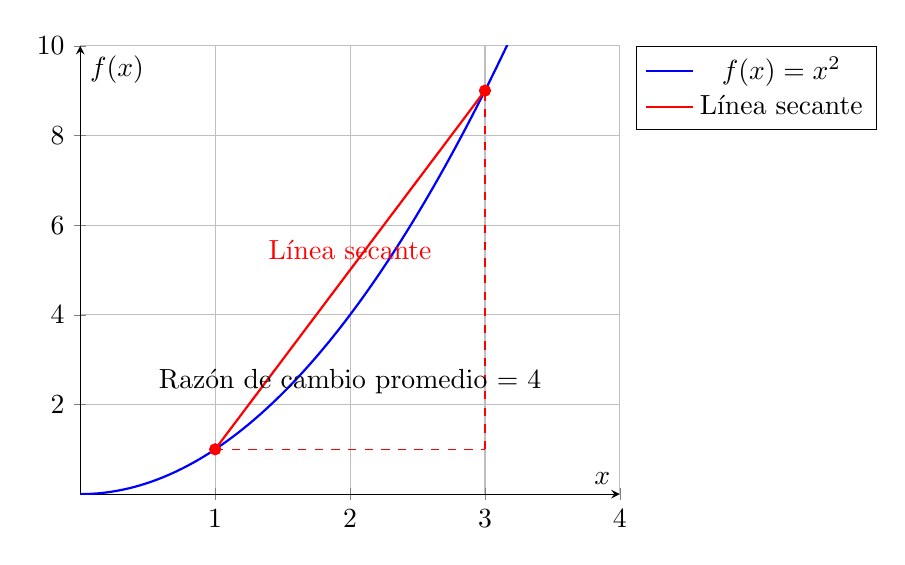
\begin{tikzpicture}
        \begin{axis}[
            axis lines=middle,
            xlabel={$x$},
            ylabel={$f(x)$},
            xmin=0, xmax=4,
            ymin=0, ymax=10,
            samples=100,
            domain=0:4,
            legend pos=outer north east,
            grid=both
        ]
        % Graficar la función f(x) = x^2
        \addplot[blue, thick] {x^2} 
            node[pos=0.9, above right] {$f(x) = x^2$};
        
        % Graficar la línea entre los puntos (1, f(1)) y (3, f(3))
        \addplot[red, thick] coordinates {(1,1) (3,9)}
            node[pos=0.5, above] {Línea secante};
        
        % Añadir una línea horizontal punteada
        \addplot[red, dashed] coordinates {(1,1) (3,1)};
        \addplot[red, dashed] coordinates {(3,1) (3,9)};
        
        % Añadir puntos en (1, f(1)) y (3, f(3))
        \addplot[red, mark=*, only marks] coordinates {(1,1) (3,9)};
        
        % Etiquetas
        \node at (2, 2.5) {Razón de cambio promedio = 4};
        
        % Leyenda
        \legend{$f(x) = x^2$, Línea secante}
        \end{axis}
    \end{tikzpicture}
\end{center}
\end{example}

\subsection{Razones de cambio y su cuantificación}


La razón de cambio instantánea en un punto \(x\) se obtiene calculando la derivada de la función en ese punto. La derivada de una función \(f(x)\) en un punto \(x_0\) proporciona la pendiente de la línea tangente a la función en ese punto.

\[
\text{Razón de cambio instantánea en } x = x_0 \text{ es } f'(x_0)
\]

\subsection{Ejemplo}
Para la función \(f(x) = x^2\), la derivada es \(f'(x) = 2x\). La razón de cambio instantánea en \(x = 2\) es:

\[
f'(2) = 2 \cdot 2 = 4
\]

A continuación, se muestra la gráfica que ilustra la razón de cambio instantánea.

\begin{center}
    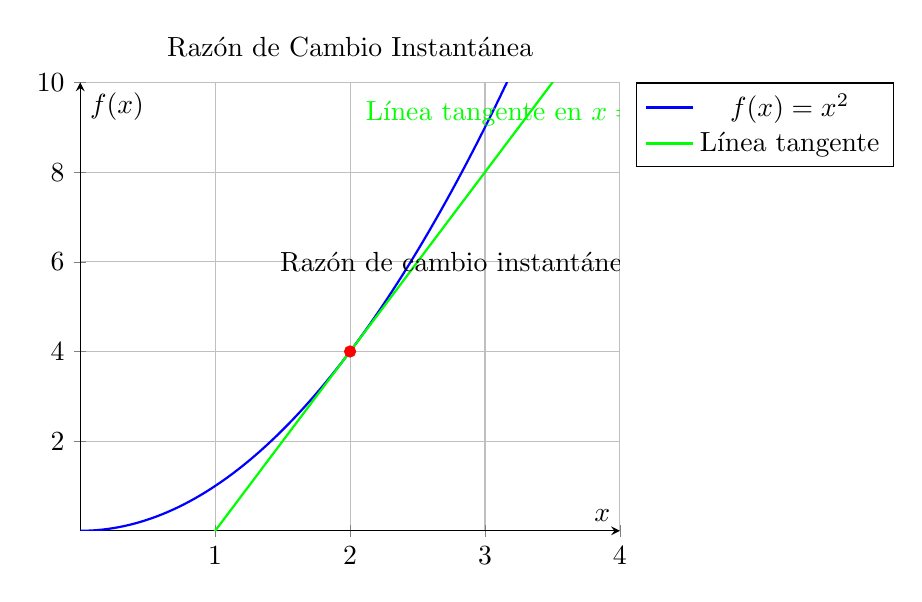
\begin{tikzpicture}
        \begin{axis}[
            axis lines=middle,
            xlabel={$x$},
            ylabel={$f(x)$},
            xmin=0, xmax=4,
            ymin=0, ymax=10,
            samples=100,
            domain=0:4,
            grid=both,
            legend pos=outer north east,
            title={Razón de Cambio Instantánea}
        ]
        % Graficar la función f(x) = x^2
        \addplot[blue, thick] {x^2} 
            node[pos=0.9, above right] {$f(x) = x^2$};
        
        % Graficar la línea tangente en x = 2
        \addplot[green, thick, domain=0:4] {4*x -4}
            node[pos=0.8, above] {Línea tangente en $x=2$};
        
        % Añadir puntos en (1, f(1)) y (3, f(3))
        \addplot[red, mark=*, only marks] coordinates {(2,4)};
        
        % Etiquetas
        \node at (3, 6) {Razón de cambio instantánea = 4};
        
        % Leyenda
        \legend{$f(x) = x^2$, Línea tangente}
        \end{axis}
    \end{tikzpicture}
\end{center}



\subsection{Razones de cambio, pendientes y curvas}
\subsection{Pendientes}

La pendiente de una línea describe su inclinación. En el contexto de funciones matemáticas, las pendientes se relacionan con las razones de cambio:

\subsubsection{Pendiente de una Línea Secante}

La pendiente de la línea secante entre dos puntos \((x_1, f(x_1))\) y \((x_2, f(x_2))\) es equivalente a la razón de cambio promedio entre esos puntos. Se calcula como:

\[
\text{Pendiente de la línea secante} = \frac{f(x_2) - f(x_1)}{x_2 - x_1}
\]

Esta pendiente mide el cambio promedio de la función entre los dos puntos.

\subsubsection{Pendiente de una Línea Tangente}

La pendiente de la línea tangente en un punto específico se determina por la derivada de la función en ese punto. La derivada \( f'(x) \) proporciona la pendiente de la línea tangente en \( x = x_0 \):

\[
\text{Pendiente de la línea tangente en } x = x_0 \text{ es } f'(x_0)
\]

La línea tangente muestra el cambio instantáneo de la función en ese punto.

\subsection{Curvas}

Las curvas representan funciones que no son lineales. Para analizar el comportamiento de las curvas, se consideran dos conceptos importantes:

\subsubsection{Razón de Cambio en Curvas}

En una curva, la razón de cambio promedio entre dos puntos se representa por la pendiente de la línea secante entre esos puntos. La razón de cambio instantánea en una curva se representa por la pendiente de la línea tangente en un punto específico, que se obtiene a través de la derivada.

\subsubsection{Curvatura}

La curvatura de una función mide cómo se desvía la curva de una línea recta. En cálculo, esto se analiza a través de la segunda derivada de la función. La segunda derivada de \( f(x) \), denotada como \( f''(x) \), proporciona información sobre la concavidad de la función:

\[
\text{Si } f''(x) > 0, \text{ la curva es cóncava hacia arriba.}
\]

\[
\text{Si } f''(x) < 0, \text{ la curva es cóncava hacia abajo.}
\]

La segunda derivada indica la velocidad a la que cambia la pendiente de la función.





\subsection{Cálculo de razones de cambio instantáneas}
Para calcular la razón de cambio instantánea, sigue estos pasos:

\subsubsection{Encuentra la Derivada de la Función}

La derivada de una función \( f(x) \), denotada como \( f'(x) \), proporciona la razón de cambio instantánea en cualquier punto \( x \). Algunas de las reglas básicas para encontrar la derivada son:

\begin{itemize}
    \item Derivada de una constante: Si \( f(x) = c \), entonces \( f'(x) = 0 \).
    \item Derivada de \( x^n \): Si \( f(x) = x^n \), entonces \( f'(x) = n \cdot x^{n-1} \).
    \item Derivada de una suma: Si \( f(x) = g(x) + h(x) \), entonces \( f'(x) = g'(x) + h'(x) \).
    \item Derivada de un producto: Si \( f(x) = g(x) \cdot h(x) \), entonces \( f'(x) = g'(x) \cdot h(x) + g(x) \cdot h'(x) \).
    \item Derivada de un cociente: Si \( f(x) = \frac{g(x)}{h(x)} \), entonces \( f'(x) = \frac{g'(x) \cdot h(x) - g(x) \cdot h'(x)}{h(x)^2} \).
\end{itemize}

\subsubsection{Evalúa la Derivada en el Punto Deseado}

Una vez que tengas la derivada \( f'(x) \), evalúala en el punto específico \( x = x_0 \) donde deseas encontrar la razón de cambio instantánea. Esto se hace sustituyendo \( x_0 \) en la derivada.

\begin{example}
    Consideremos la función \( f(x) = x^2 \). Calcularemos la razón de cambio instantánea en \( x = 3 \).

\subsubsection{Encuentra la Derivada}

La derivada de \( f(x) = x^2 \) es:

\[
f'(x) = 2x
\]

Evalúa la Derivada en \( x = 3 \)

Sustituimos \( x = 3 \) en la derivada:

\[
f'(3) = 2 \cdot 3 = 6
\]

Por lo tanto, la razón de cambio instantánea de la función \( f(x) = x^2 \) en el punto \( x = 3 \) es 6.

\end{example}


\section{Funciones} % 12 clases
\subsection{Concepto de función. Notación y clasificación:}
\begin{definition}[Función]
    Una \textbf{función} es una relación entre un conjunto de \textbf{entrada} (o \textbf{dominio}) y un conjunto de \textbf{salida} (o \textbf{contradominio}) en la cual a cada elemento del dominio le corresponde un único elemento del contradominio. Formalmente, una función \( f \) de un conjunto \( X \) a un conjunto \( Y \) se denota como:

\begin{equation}
    f: X \rightarrow Y
\end{equation}

y para cada \( x \in X \), \( f(x) \) es el elemento correspondiente en \( Y \). 
\end{definition}

\begin{notation}
    La notación estándar para una función es \( f(x) \), donde \( x \) es la variable independiente y \( f(x) \) es el valor de la función para ese valor de \( x \)
\end{notation}
\begin{example}
    Si \( f(x) = x^2 \), entonces para \( x = 3 \), \( f(3) = 9 \).
\end{example}

\begin{itemize}
    \item \textbf{Funciones Algebraicas:} Son funciones que pueden expresarse usando operaciones algebraicas básicas como suma, resta, multiplicación, división, y raíces. Ejemplos incluyen polinomios y fracciones algebraicas.
    \item \textbf{Funciones Trigonométricas:} Incluyen funciones como el seno, coseno y tangente, que están relacionadas con los ángulos y triángulos.
    \item \textbf{Funciones Exponenciales y Logarítmicas:} Funciones como \( f(x) = e^x \) o \( g(x) = \log(x) \).
    \item \textbf{Funciones Racionales:} Son funciones que pueden expresarse como el cociente de dos polinomios. Ejemplo: \( \frac{p(x)}{q(x)} \).
    \item \textbf{Funciones Irracionales:} Incluyen funciones que contienen raíces de variables. Ejemplo: \( f(x) = \sqrt{x} \).
    \item \textbf{Funciones Especiales:} Como la función paso, función gama, entre otras.
\end{itemize}

\subsubsection{Algebraicas: racionales e irracionales.}


\begin{itemize}
    \item \textbf{Funciones Algebraicas:} Son funciones que pueden expresarse usando operaciones algebraicas básicas como suma, resta, multiplicación, división, y raíces. Ejemplos incluyen polinomios y fracciones algebraicas.
    \begin{figure}[h!]
        \centering
        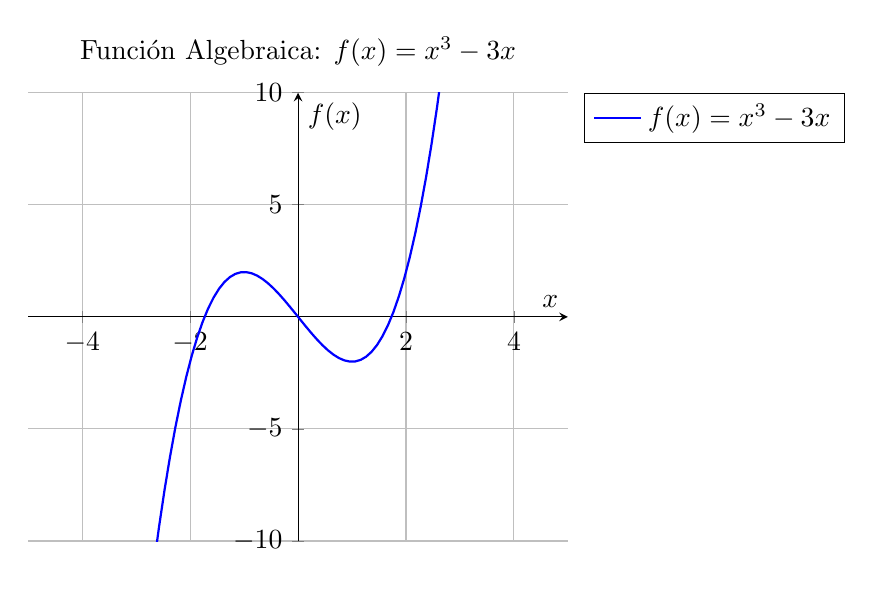
\begin{tikzpicture}
        \begin{axis}[
            axis lines=middle,
            xlabel={$x$},
            ylabel={$f(x)$},
            xmin=-5, xmax=5,
            ymin=-10, ymax=10,
            samples=100,
            domain=-5:5,
            legend pos=outer north east,
            grid=both,
            title={Función Algebraica: $f(x) = x^3 - 3x$}
        ]
        \addplot[blue, thick] {x^3 - 3*x};
        \legend{$f(x) = x^3 - 3x$}
        \end{axis}
        \end{tikzpicture}
        \caption{Gráfica de la función algebraica $f(x) = x^3 - 3x$.}
        \end{figure}
    

    \item \textbf{Funciones Racionales:} Son funciones que pueden expresarse como el cociente de dos polinomios. Ejemplo: \( \frac{p(x)}{q(x)} \).
    \begin{figure}[h!]
        \centering
        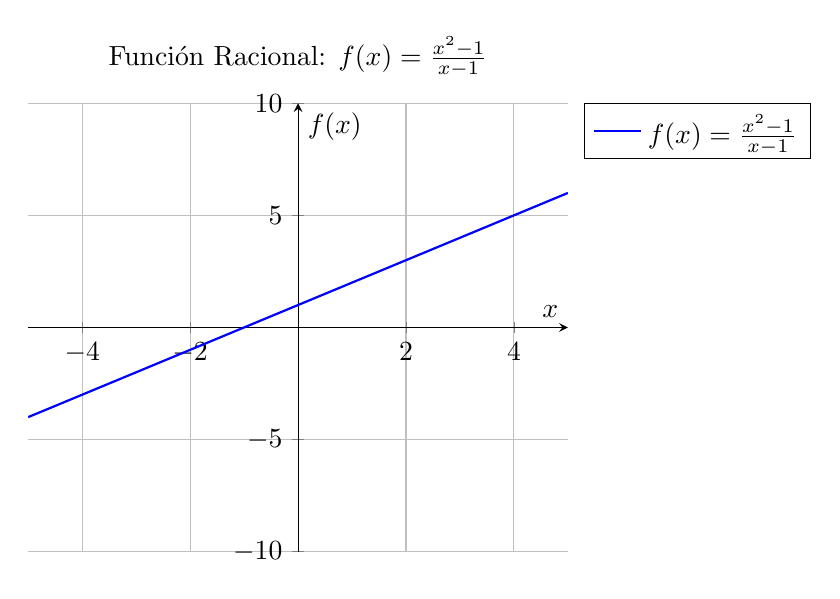
\begin{tikzpicture}
        \begin{axis}[
            axis lines=middle,
            xlabel={$x$},
            ylabel={$f(x)$},
            xmin=-5, xmax=5,
            ymin=-10, ymax=10,
            samples=100,
            domain=-5:5,
            restrict y to domain=-10:10,
            legend pos=outer north east,
            grid=both,
            title={Función Racional: $f(x) = \frac{x^2 - 1}{x - 1}$}
        ]
        \addplot[blue, thick] {(x^2 - 1) / (x - 1)};
        \legend{$f(x) = \frac{x^2 - 1}{x - 1}$}
        \end{axis}
        \end{tikzpicture}
        \caption{Gráfica de la función racional $f(x) = \frac{x^2 - 1}{x - 1}$.}
        \end{figure}
        \newpage
    \item \textbf{Funciones Irracionales:} Incluyen funciones que contienen raíces de variables. Ejemplo: \( f(x) = \sqrt{x} \).
    \begin{figure}[h!]
        \centering
        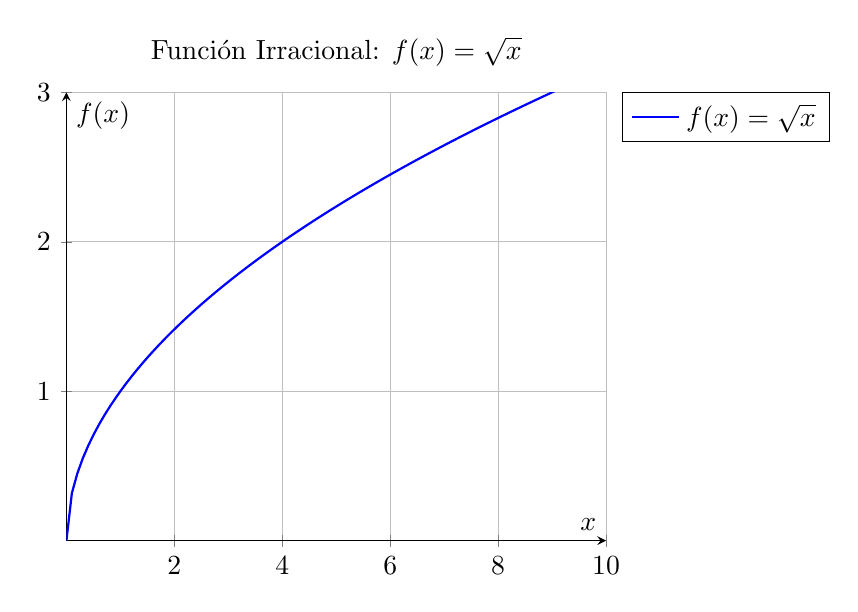
\begin{tikzpicture}
        \begin{axis}[
            axis lines=middle,
            xlabel={$x$},
            ylabel={$f(x)$},
            xmin=0, xmax=10,
            ymin=0, ymax=3,
            samples=100,
            domain=0:10,
            legend pos=outer north east,
            grid=both,
            title={Función Irracional: $f(x) = \sqrt{x}$}
        ]
        \addplot[blue, thick] {sqrt(x)};
        \legend{$f(x) = \sqrt{x}$}
        \end{axis}
        \end{tikzpicture}
        \caption{Gráfica de la función irracional $f(x) = \sqrt{x}$.}
        \end{figure}
\end{itemize}


\subsubsection{Trascendentes: trigonométricas, logarítmicas y exponenciales}

\begin{itemize}
    \item \textbf{Funciones Trigonométricas:} Incluyen funciones como el seno, coseno y tangente, que están relacionadas con los ángulos y triángulos.
    \begin{figure}[h!]
        \centering
        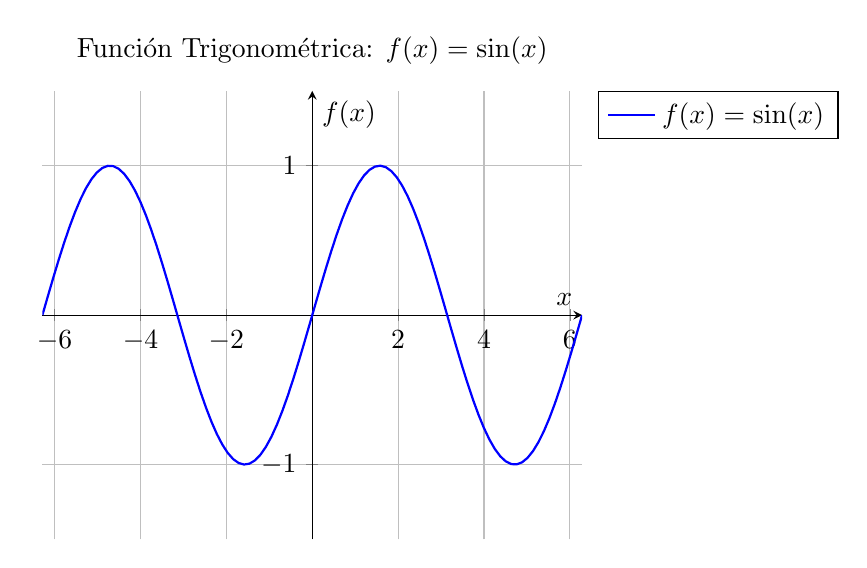
\begin{tikzpicture}
        \begin{axis}[
            axis lines=middle,
            xlabel={$x$},
            ylabel={$f(x)$},
            xmin=-2*pi, xmax=2*pi,
            ymin=-1.5, ymax=1.5,
            samples=100,
            domain=-2*pi:2*pi,
            legend pos=outer north east,
            grid=both,
            title={Función Trigonométrica: $f(x) = \sin(x)$}
        ]
        \addplot[blue, thick] {sin(deg(x))};
        \legend{$f(x) = \sin(x)$}
        \end{axis}
        \end{tikzpicture}
        \caption{Gráfica de la función trigonométrica $f(x) = \sin(x)$.}
        \end{figure}
        \item \textbf{Funciones Exponenciales y Logarítmicas:} Funciones como \( f(x) = e^x \) o \( g(x) = \log(x) \).
    
    \begin{figure}[h!]
        \centering
        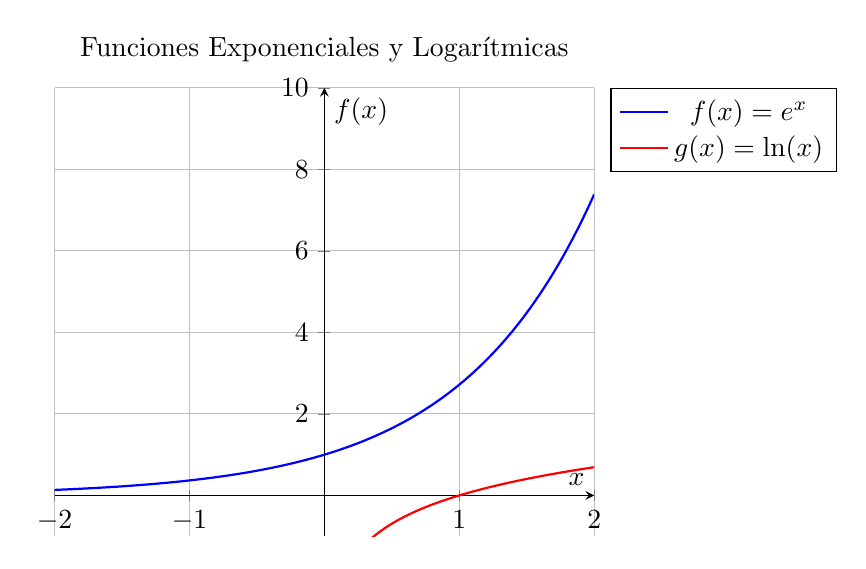
\begin{tikzpicture}
        \begin{axis}[
            axis lines=middle,
            xlabel={$x$},
            ylabel={$f(x)$},
            xmin=-2, xmax=2,
            ymin=-1, ymax=10,
            samples=100,
            domain=-2:2,
            legend pos=outer north east,
            grid=both,
            title={Funciones Exponenciales y Logarítmicas}
        ]
        \addplot[blue, thick] {exp(x)};
        \addplot[red, thick, domain=0:2] {ln(x)};
        \addlegendentry{$f(x) = e^x$}
        \addlegendentry{$g(x) = \ln(x)$}
        \end{axis}
        \end{tikzpicture}
        \caption{Gráficas de $f(x) = e^x$ y $g(x) = \ln(x)$.}
        \end{figure}
\end{itemize}



\subsection{Elementos esenciales de una función (dominio y contra dominio)}

\subsubsection{Dominio}

\begin{definition}[Dominio]
    Es el conjunto de todos los valores de entrada (valores de la variable independiente) para los cuales la función está definida. Es decir, el dominio representa el conjunto de todos los posibles valores que pueden ser utilizados como entrada para la función.

Si \( f: A \to B \) es una función que asigna cada elemento de \( A \) a un único elemento en \( B \), entonces el dominio de \( f \) es el conjunto \( A \).
\begin{equation}
    \text{Dominio}(f) = \{ x \in A \mid f(x) \text{ está definido} \}
\end{equation}
\end{definition}
\begin{example}
    Para la función \( f(x) = \frac{1}{x} \), el dominio está definido para todos los números reales excepto \( x = 0 \), ya que la división por cero no está definida.
\end{example}
\subsubsection{Contradominio}
\begin{definition}[Contradominio o Rango]
    Es el conjunto de todos los posibles valores de salida (valores de la variable dependiente) que la función puede tomar. A diferencia del rango (o imagen) de la función, que es el conjunto real de valores que efectivamente toma la función, el contradominio es el conjunto de valores que la función podría tomar, definido por la función misma o por el contexto en el que se utiliza.

Si \( f: A \to B \), el contradominio de \( f \) es el conjunto \( B \), que representa todos los posibles valores de salida.
\begin{equation}
    \text{Contradominio}(f) = B
\end{equation}
\end{definition}
\begin{example}
    Para la función \( f(x) = x^2 \) definida en los números reales, el contradominio es el conjunto de todos los números reales no negativos, es decir, \( [0, \infty) \), aunque el rango exacto también sería \( [0, \infty) \).
\end{example}

\begin{problem}[Encontrar el dominio y rango]
    Consideremos la función \( f(x) = \sqrt{x-2} \)

\begin{itemize}
    \item \textbf{Dominio:} Para que \( f(x) = \sqrt{x-2} \) esté definida, el argumento de la raíz cuadrada debe ser mayor o igual a cero. Por lo tanto, \( x-2 \geq 0 \) o \( x \geq 2 \). El dominio de \( f \) es \( [2, \infty) \).
    \item \textbf{Contradominio:} Dado que la función raíz cuadrada siempre produce valores no negativos, el contradominio de \( f \) es \( [0, \infty) \).
\end{itemize}

\end{problem}

\subsection{Evaluación de funciones y Gráficas de funciones: constante, lineal, cuadrática}

\subsubsection{Dominio}

El \textbf{dominio} de una función es el conjunto de todos los posibles valores de entrada \( x \) para los cuales la función está definida.

\begin{itemize}
    \item \textbf{Función Constante:} Para una función constante \( f(x) = c \), donde \( c \) es una constante, el dominio es el conjunto de todos los números reales, ya que la función está definida para cualquier valor de \( x \).
    
    \item \textbf{Función Lineal:} Para una función lineal \( f(x) = mx + b \), donde \( m \) y \( b \) son constantes, el dominio también es el conjunto de todos los números reales, ya que las funciones lineales están definidas para cualquier \( x \).

    \item \textbf{Función Cuadrática:} Para una función cuadrática \( f(x) = ax^2 + bx + c \), el dominio es el conjunto de todos los números reales. Las funciones cuadráticas están definidas para cualquier valor de \( x \).

    \item \textbf{Función Racional:} Para una función racional \( f(x) = \frac{p(x)}{q(x)} \), donde \( p(x) \) y \( q(x) \) son polinomios, el dominio es el conjunto de todos los números reales excepto los valores de \( x \) que hacen que \( q(x) = 0 \).
    
    \item \textbf{Función Radicada:} Para una función radicada \( f(x) = \sqrt{x - a} \), el dominio es el conjunto de todos los \( x \) tales que \( x - a \geq 0 \), es decir, \( x \geq a \).
\end{itemize}

\subsubsection{Rango}

El \textbf{rango} de una función es el conjunto de todos los posibles valores de salida \( y \) que la función puede tomar.

\begin{itemize}
    \item \textbf{Función Constante:} El rango de una función constante \( f(x) = c \) es simplemente el conjunto que contiene el valor \( c \), es decir, \(\{c\}\).

    \item \textbf{Función Lineal:} El rango de una función lineal \( f(x) = mx + b \) es el conjunto de todos los números reales, ya que la función lineal puede tomar cualquier valor real.

    \item \textbf{Función Cuadrática:} El rango de una función cuadrática \( f(x) = ax^2 + bx + c \) depende del coeficiente \( a \):
    \begin{itemize}
        \item Si \( a > 0 \), el rango es \([k, \infty)\), donde \( k \) es el valor mínimo de la función (el vértice de la parábola).
        \item Si \( a < 0 \), el rango es \((-\infty, k]\), donde \( k \) es el valor máximo de la función.
    \end{itemize}
    
    \item \textbf{Función Racional:} El rango de una función racional puede ser más complicado de determinar y a menudo requiere la resolución de ecuaciones y el análisis del comportamiento asintótico.

    \item \textbf{Función Radicada:} Para una función radicada \( f(x) = \sqrt{x - a} \), el rango es \([0, \infty)\), ya que la raíz cuadrada siempre da valores no negativos.
\end{itemize}



\subsection{Gráficas de funciones algebraicas y trascendentes.}

Una función constante tiene la forma \( f(x) = c \). Su gráfica es una línea horizontal en \( y = c \). La gráfica de una función constante se muestra a continuación:

\begin{figure}[h!]
\centering
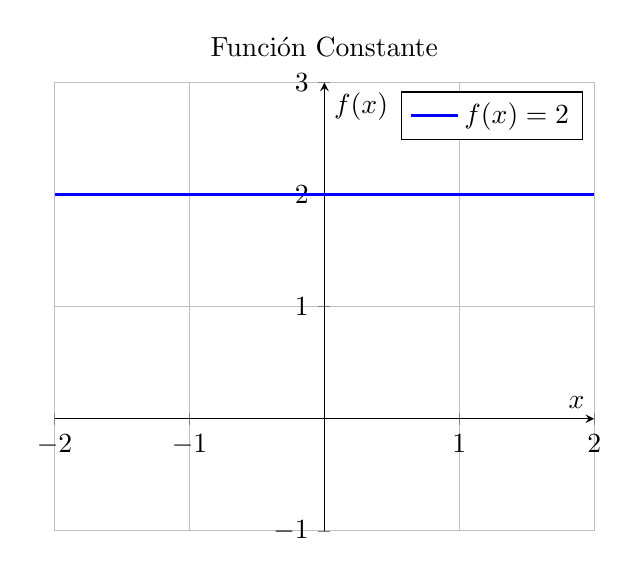
\begin{tikzpicture}
\begin{axis}[
    axis lines=middle,
    xlabel={$x$},
    ylabel={$f(x)$},
    xmin=-2, xmax=2,
    ymin=-1, ymax=3,
    samples=100,
    domain=-2:2,
    grid=both,
    title={Función Constante}
]
\addplot[blue, thick] {2};
\addlegendentry{$f(x) = 2$}
\end{axis}
\end{tikzpicture}
\caption{Gráfica de la función constante $f(x) = 2$.}
\end{figure}

\subsection{Función Lineal}

Una función lineal tiene la forma \( f(x) = mx + b \). Su gráfica es una línea recta. La pendiente \( m \) determina la inclinación de la línea, y \( b \) es la intersección con el eje \( y \). La gráfica de una función lineal se muestra a continuación:

\begin{figure}[h!]
\centering
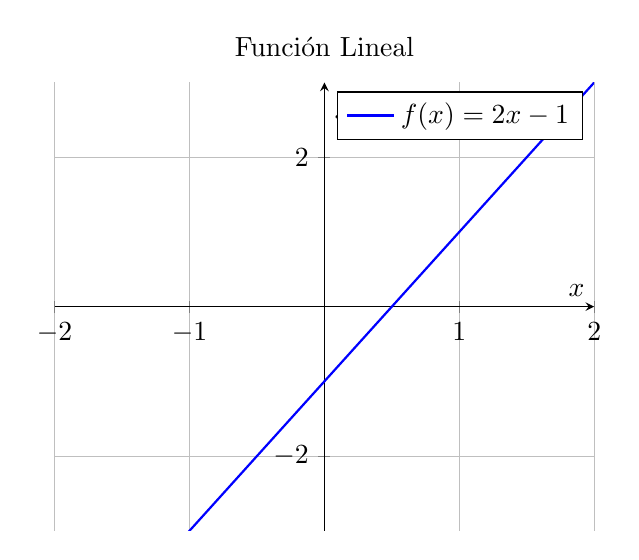
\begin{tikzpicture}
\begin{axis}[
    axis lines=middle,
    xlabel={$x$},
    ylabel={$f(x)$},
    xmin=-2, xmax=2,
    ymin=-3, ymax=3,
    samples=100,
    domain=-2:2,
    grid=both,
    title={Función Lineal}
]
\addplot[blue, thick] {2*x - 1};
\addlegendentry{$f(x) = 2x - 1$}
\end{axis}
\end{tikzpicture}
\caption{Gráfica de la función lineal $f(x) = 2x - 1$.}
\end{figure}

\subsection{Función Cuadrática}

Una función cuadrática tiene la forma \( f(x) = ax^2 + bx + c \). Su gráfica es una parábola. El parámetro \( a \) determina la dirección en la que se abre la parábola (hacia arriba si \( a > 0 \), hacia abajo si \( a < 0 \)). La gráfica de una función cuadrática se muestra a continuación:

\begin{figure}[h!]
\centering
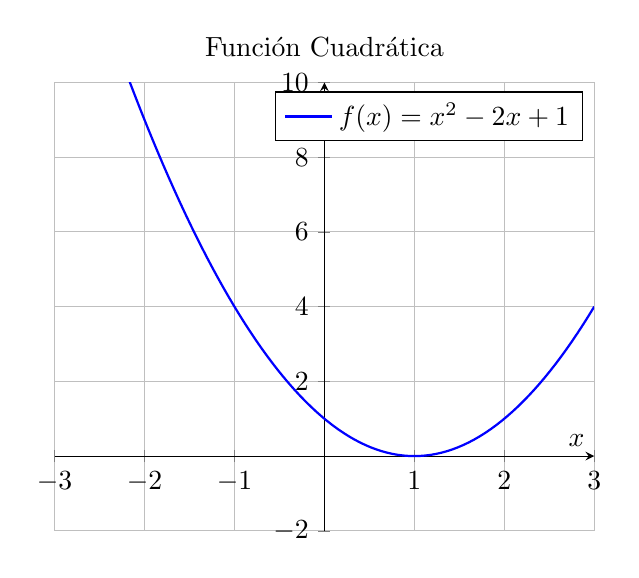
\begin{tikzpicture}
\begin{axis}[
    axis lines=middle,
    xlabel={$x$},
    ylabel={$f(x)$},
    xmin=-3, xmax=3,
    ymin=-2, ymax=10,
    samples=100,
    domain=-3:3,
    grid=both,
    title={Función Cuadrática}
]
\addplot[blue, thick] {x^2 - 2*x + 1};
\addlegendentry{$f(x) = x^2 - 2x + 1$}
\end{axis}
\end{tikzpicture}
\caption{Gráfica de la función cuadrática $f(x) = x^2 - 2x + 1$.}
\end{figure}


\subsection{Funciones definidas por intervalos.}
Una función definida por intervalos se define mediante diferentes expresiones en diferentes intervalos de su dominio. Por ejemplo:

\[
f(x) = 
\begin{cases} 
x^2 & \text{si } x \leq 0 \\
2x + 1 & \text{si } x > 0 
\end{cases}
\]

Para graficar esta función, se grafica cada parte de la función en el intervalo correspondiente.



\subsection{Operaciones con funciones (suma, resta, multiplicación, división y composición).}
Dado dos funciones \( f \) y \( g \), las operaciones básicas incluyen:

\begin{itemize}
    \item \textbf{Suma:} \( (f + g)(x) = f(x) + g(x) \)
    \item \textbf{Resta:} \( (f - g)(x) = f(x) - g(x) \)
    \item \textbf{Multiplicación:} \( (f \cdot g)(x) = f(x) \cdot g(x) \)
    \item \textbf{División:} \( \left(\frac{f}{g}\right)(x) = \frac{f(x)}{g(x)} \), para \( g(x) \neq 0 \)
    \item \textbf{Composición:} \( (f \circ g)(x) = f(g(x)) \)
\end{itemize}


\subsection{Función inversa.}
La inversa de una función \( f \), denotada como \( f^{-1} \), es una función tal que:
\begin{align}
    &f(f^{-1}(x)) = x \\
    &f^{-1}(f(x)) = x
\end{align}

Para encontrar la inversa de una función, intercambia \( x \) y \( y \) en la ecuación de la función original y resuelve para \( y \).

\section{Límites y continuidad} % 9 clases
El límite de una función es un concepto fundamental en el cálculo que describe el comportamiento de una función a medida que la variable independiente se acerca a un punto específico. En términos simples, el límite de una función \( f(x) \) en un punto \( a \) examina el valor al que \( f(x) \) se aproxima cuando \( x \) se acerca a \( a \).
\subsection{Concepto de límite de una función}


\begin{definition}[Limite]
    El límite de una función \( f(x) \) cuando \( x \) tiende a \( a \) se denota como
\[
\lim_{x \to a} f(x).
\]
Formalmente, se dice que
\[
\lim_{x \to a} f(x) = L
\]
si para cualquier número positivo \( \epsilon \), por pequeño que sea, existe un número positivo \( \delta \) tal que siempre que \( 0 < |x - a| < \delta \), se cumple
\[
|f(x) - L| < \epsilon.
\]
\end{definition}

\subsection{Interpretación Gráfica}

Gráficamente, el límite de una función en un punto \( a \) representa el valor al que la gráfica de la función se aproxima a medida que \( x \) se acerca a \( a \). Esto no necesariamente implica que \( f(x) \) esté definido en \( x = a \), sino que \( f(x) \) se comporta de manera predecible a medida que \( x \) se acerca a \( a \).

\begin{figure}[h!]
    \centering
    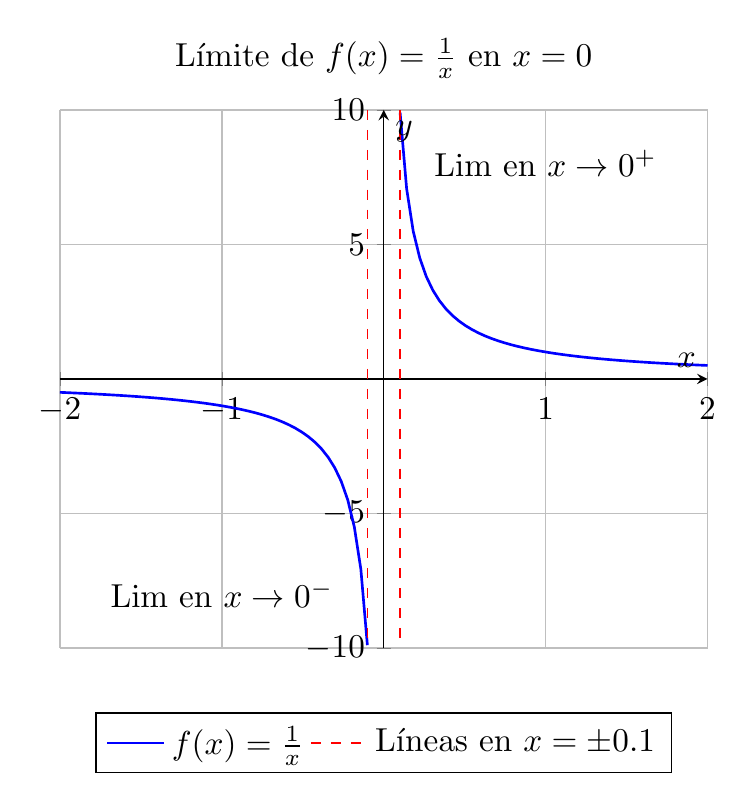
\begin{tikzpicture}[scale=1.2] % Aumenta el tamaño de la gráfica
    \begin{axis}[
        axis lines=middle,
        xlabel={$x$},
        ylabel={$y$},
        xmin=-2, xmax=2,
        ymin=-10, ymax=10,
        samples=100,
        domain=-2:2,
        restrict y to domain=-10:10,
        grid=both,
        title={Límite de $f(x) = \frac{1}{x}$ en $x = 0$},
        legend style={
            at={(0.5,-0.12)}, % Posiciona la leyenda debajo de la gráfica
            anchor=north,
            legend columns=-1
        }
    ]
    % Función f(x) = 1/x
    \addplot[blue, thick] {1/x};
    \addlegendentry{$f(x) = \frac{1}{x}$}
    
    % Líneas verticales en x = -0.1 y x = 0.1 para mostrar el comportamiento cerca de x = 0
    \addplot[red, dashed] coordinates {(-0.1, 10) (-0.1, -10)};
    \addplot[red, dashed] coordinates {(0.1, 10) (0.1, -10)};
    \addlegendentry{Líneas en $x = \pm 0.1$}
    
    % Etiquetas
    \node at (1, 8) {Lim en $x \to 0^+$};
    \node at (-1, -8) {Lim en $x \to 0^-$};
    
    \end{axis}
    \end{tikzpicture}
    \caption{Gráfica de la función $f(x) = \frac{1}{x}$ mostrando cómo se aproxima a $\infty$ o $-\infty$ cuando $x$ se acerca a 0 desde la derecha o desde la izquierda.}
    \end{figure}
    

    

\subsubsection{Límite Finito}

Considera la función \( f(x) = 2x + 3 \). Queremos encontrar
\[
\lim_{x \to 1} f(x).
\]
Sustituyendo \( x = 1 \) en la función,
\[
\lim_{x \to 1} (2x + 3) = 2 \cdot 1 + 3 = 5.
\]
Por lo tanto, el límite es 5.

\subsubsection{Límite Infinito}

Para la función \( f(x) = \frac{1}{x} \), el límite cuando \( x \) tiende a 0 no está definido de manera finita. Sin embargo, podemos analizar el comportamiento de la función cuando \( x \) se acerca a 0 desde la derecha y desde la izquierda. En este caso, tenemos:
\[
\lim_{x \to 0^+} \frac{1}{x} = +\infty
\]
y
\[
\lim_{x \to 0^-} \frac{1}{x} = -\infty.
\]

\subsection{Límites Laterales}

Si el límite de \( f(x) \) existe cuando \( x \) se acerca a \( a \) desde la izquierda (denotado \( \lim_{x \to a^-} f(x) \)) y desde la derecha (denotado \( \lim_{x \to a^+} f(x) \)), y ambos límites son iguales, entonces el límite en \( x = a \) existe y es igual a este valor común:
\[
\lim_{x \to a} f(x) = L \text{ si } \lim_{x \to a^-} f(x) = \lim_{x \to a^+} f(x) = L.
\]
\subsection{Teoremas sobre límites}

\subsubsection{Teorema del Límite de una Suma}

Si \( \lim_{x \to a} f(x) = L \) y \( \lim_{x \to a} g(x) = M \), entonces el límite de la suma de las funciones es la suma de los límites:
\[
\lim_{x \to a} \left( f(x) + g(x) \right) = L + M.
\]

\subsubsection{Teorema del Límite de un Producto}

Si \( \lim_{x \to a} f(x) = L \) y \( \lim_{x \to a} g(x) = M \), entonces el límite del producto de las funciones es el producto de los límites:
\[
\lim_{x \to a} \left( f(x) \cdot g(x) \right) = L \cdot M.
\]

\subsubsection{Teorema del Límite de un Cociente}

Si \( \lim_{x \to a} f(x) = L \) y \( \lim_{x \to a} g(x) = M \), y \( M \neq 0 \), entonces el límite del cociente de las funciones es el cociente de los límites:
\[
\lim_{x \to a} \left( \frac{f(x)}{g(x)} \right) = \frac{L}{M}.
\]

\subsubsection{Teorema del Límite de una Función Compuesta}

Si \( \lim_{x \to a} f(x) = L \) y \( \lim_{x \to L} g(x) = M \), entonces el límite de la composición de las funciones es el límite de la función exterior evaluado en el límite de la función interior:
\[
\lim_{x \to a} g(f(x)) = M.
\]

\subsubsection{Teorema del Límite de una Función Polinómica}

Los límites de las funciones polinómicas se pueden calcular directamente evaluando el valor de la variable en el punto del límite:
\[
\lim_{x \to a} (p(x)) = p(a),
\]
donde \( p(x) \) es un polinomio.

\subsubsection{Teorema del Límite de Funciones Racionales}

Si \( \lim_{x \to a} p(x) \) y \( \lim_{x \to a} q(x) \) existen y \( \lim_{x \to a} q(x) \neq 0 \), entonces:
\[
\lim_{x \to a} \frac{p(x)}{q(x)} = \frac{\lim_{x \to a} p(x)}{\lim_{x \to a} q(x)}.
\]

\subsubsection{Teorema del Límite en el Infinito}

Si \( \lim_{x \to \infty} f(x) = L \), entonces para cualquier \( \epsilon > 0 \), existe un número \( N \) tal que si \( x > N \), entonces \( |f(x) - L| < \epsilon \).

\subsection{Cálculo de límites.}

\subsubsection{Cálculo de Límites por Sustitución Directa}

Si la función \( f(x) \) es continua en \( x = a \), entonces:
\[
\lim_{x \to a} f(x) = f(a)
\]
Por ejemplo, para la función polinómica \( f(x) = 3x^2 - 2x + 1 \), simplemente sustituimos \( x = a \) para encontrar el límite:
\[
\lim_{x \to 2} (3x^2 - 2x + 1) = 3(2)^2 - 2(2) + 1 = 9.
\]

\subsubsection{Cálculo de Límites para Funciones Racionales}

Para una función racional \( f(x) = \frac{p(x)}{q(x)} \), donde \( p(x) \) y \( q(x) \) son polinomios, el límite se puede calcular simplificando la expresión:
\[
\lim_{x \to a} \frac{p(x)}{q(x)} = \frac{\lim_{x \to a} p(x)}{\lim_{x \to a} q(x)}
\]
si \( \lim_{x \to a} q(x) \neq 0 \). 

Por ejemplo, para la función \( f(x) = \frac{x^2 - 4}{x - 2} \):
\[
\lim_{x \to 2} \frac{x^2 - 4}{x - 2} = \lim_{x \to 2} \frac{(x - 2)(x + 2)}{x - 2} = \lim_{x \to 2} (x + 2) = 4.
\]


Cuando enfrentamos formas indeterminadas como \( \frac{0}{0} \) o \( \frac{\infty}{\infty} \), se pueden usar métodos adicionales como la factorización, el uso de identidades trigonométricas, o la regla de L'Hôpital.

\subsection{Regla de L'Hôpital}

Si \( \lim_{x \to a} \frac{f(x)}{g(x)} \) da una forma indeterminada \( \frac{0}{0} \) o \( \frac{\infty}{\infty} \), y las derivadas \( f'(x) \) y \( g'(x) \) existen, entonces:
\[
\lim_{x \to a} \frac{f(x)}{g(x)} = \lim_{x \to a} \frac{f'(x)}{g'(x)}
\]
si el límite del cociente de las derivadas existe.

Por ejemplo, para la función \( f(x) = \frac{\sin(x)}{x} \):
\[
\lim_{x \to 0} \frac{\sin(x)}{x} \text{ da la forma indeterminada } \frac{0}{0}.
\]
Aplicamos la regla de L'Hôpital:
\[
\lim_{x \to 0} \frac{\sin(x)}{x} = \lim_{x \to 0} \frac{\cos(x)}{1} = 1.
\]

\subsubsection{Límites en el Infinito}

Para funciones que tienden al infinito, se analizan los comportamientos asintóticos. Por ejemplo, para \( f(x) = \frac{3x^2 - 2}{x^2 + 1} \):
\[
\lim_{x \to \infty} \frac{3x^2 - 2}{x^2 + 1} = \lim_{x \to \infty} \frac{3 - \frac{2}{x^2}}{1 + \frac{1}{x^2}} = 3.
\]

\subsubsection{Continuidad de funciones}

Una función se dice que es continua en un punto si no tiene interrupciones, saltos o agujeros en ese punto. Formalmente, para una función \( f(x) \), la continuidad en un punto \( a \) se define como sigue:



\subsection{Definición de Continuidad en un Punto}

Una función \( f(x) \) es continua en un punto \( a \) si se cumplen las siguientes tres condiciones:

\begin{enumerate}
    \item \textbf{La función está definida en } \( a \): \( f(a) \) debe existir.
    \item \textbf{El límite de la función cuando } \( x \) \textbf{ tiende a } \( a \) \textbf{ existe}: \[
    \lim_{x \to a} f(x) \text{ debe existir.}
    \]
    \item \textbf{El límite de la función es igual al valor de la función en } \( a \): \[
    \lim_{x \to a} f(x) = f(a).
    \]
\end{enumerate}

Si todas estas condiciones se satisfacen, entonces \( f(x) \) es continua en \( x = a \). De lo contrario, la función no es continua en \( x = a \).

\subsubsection{Tipos de Discontinuidades}

Si una función no es continua en un punto, puede presentar una de las siguientes discontinuidades:

\begin{itemize}
    \item \textbf{Discontinuidad Removible:} Ocurre cuando el límite de la función existe en el punto \( a \), pero la función no está definida en \( a \), o \( f(a) \) no es igual al límite. Gráficamente, esto se puede visualizar como un "agujero" en la gráfica de la función.
    
    \item \textbf{Discontinuidad de Salto:} Ocurre cuando el límite de la función no existe en \( a \) debido a que la función se acerca a diferentes valores desde la izquierda y desde la derecha. Gráficamente, esto se muestra como un "salto" en la gráfica.
    
    \item \textbf{Discontinuidad Infinita:} Ocurre cuando la función tiende a \( \infty \) o \( -\infty \) a medida que \( x \) se acerca al punto \( a \). Gráficamente, esto se muestra como una asíntota vertical.
\end{itemize}

\subsubsection{Continuidad en un Intervalo}

Una función \( f(x) \) es continua en un intervalo \( (a, b) \) si es continua en cada punto del intervalo. En otras palabras, para cualquier \( x \) en \( (a, b) \), \( f(x) \) debe ser continua.

\subsubsection{Propiedades de las Funciones Continuas}

\begin{itemize}
    \item \textbf{Suma, Resta y Producto:} La suma, resta y producto de funciones continuas son continuas.
    
    \item \textbf{Cociente:} El cociente de dos funciones continuas \( f(x) \) y \( g(x) \) es continua siempre que \( g(x) \neq 0 \) en el dominio de la función.
    
    \item \textbf{Composición:} La composición de dos funciones continuas \( f \) y \( g \) es continua. Si \( f \) es continua en \( x = a \) y \( g \) es continua en \( f(a) \), entonces la función compuesta \( g(f(x)) \) es continua en \( x = a \).
\end{itemize}

\subsubsection{Ejemplos de Continuidad}

\begin{itemize}
    \item \textbf{Función Polinómica:} Las funciones polinómicas son continuas en todo su dominio. Por ejemplo, \( f(x) = 3x^2 - 2x + 1 \) es continua en todos los valores de \( x \).
    
    \item \textbf{Función Racional:} La función \( f(x) = \frac{2x + 1}{x - 3} \) es continua en todo su dominio excepto en \( x = 3 \), donde tiene una discontinuidad infinita.
    
    \item \textbf{Función Trigonométrica:} Las funciones trigonométricas básicas como \( \sin(x) \) y \( \cos(x) \) son continuas en todo su dominio.
    
    \item \textbf{Función de Valor Absoluto:} La función \( f(x) = |x| \) es continua en todo su dominio, aunque tiene una discontinuidad removible en \( x = 0 \) si se considera en términos de derivadas.
\end{itemize}







\section{La derivada} % 12 clases
\subsection{Concepto de derivada de una función}

La derivada de una función en un punto es uno de los conceptos fundamentales en el cálculo diferencial. Representa la razón de cambio instantánea de la función en ese punto y se interpreta como la pendiente de la recta tangente a la curva en dicho punto.

\begin{definition}[Derivada]
    La derivada de una función $f(x)$ en un punto $x = a$ se define como el límite:
\begin{equation}
    f'(a) = \lim_{h \to 0} \frac{f(a+h) - f(a)}{h}
\end{equation}

\noindent Esta definición se conoce como \textbf{regla del cociente incremental} o \textbf{regla de los cuatro pasos}.
\end{definition}

\subsection{Interpretación geométrica y física de la derivada de una función}

Geométricamente, la derivada $f'(a)$ es la pendiente de la recta tangente a la curva $y = f(x)$ en el punto $(a, f(a))$. Si la función es diferenciable en $a$, entonces la curva es suave en ese punto, y la tangente existe y es única.

\begin{center}
    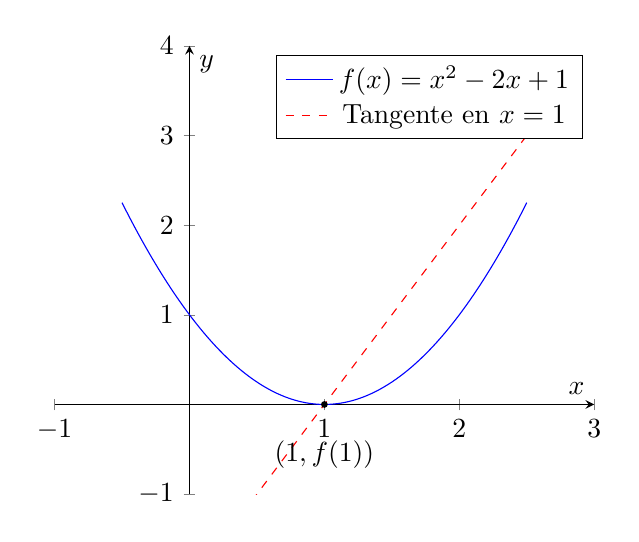
\begin{tikzpicture}
        \begin{axis}[
            axis lines = middle,
            xlabel = $x$,
            ylabel = {$y$},
            xmin = -1, xmax = 3,
            ymin = -1, ymax = 4,
            samples = 100
        ]
        \addplot [
            domain=-0.5:2.5, 
            samples=100, 
            color=blue,
        ]
        {x^2 - 2*x + 1};
        \addlegendentry{$f(x) = x^2 - 2x + 1$}
        
        \addplot [
            domain=-0.5:2.5, 
            samples=100, 
            color=red,
            dashed
        ]
        {2*(x - 1)};
        \addlegendentry{Tangente en $x=1$}
        
        \draw [fill] (axis cs:1,0) circle [radius=1pt];
        \node at (axis cs:1,-0.3) [anchor=north] {$(1, f(1))$};
        \end{axis}
    \end{tikzpicture}
\end{center}

\subsection*{Ejemplo}
Consideremos la función $f(x) = x^2$. La derivada de $f(x)$ en cualquier punto $x$ es:
\begin{equation*}
    f'(x) = \lim_{h \to 0} \frac{(x+h)^2 - x^2}{h} = \lim_{h \to 0} \frac{x^2 + 2xh + h^2 - x^2}{h} = \lim_{h \to 0} (2x + h) = 2x
\end{equation*}
En particular, en $x = 1$, la derivada es $f'(1) = 2 \times 1 = 2$, que corresponde a la pendiente de la tangente en ese punto.

En física, la derivada de la posición de una partícula respecto al tiempo representa su velocidad instantánea. Si $s(t)$ es la posición de una partícula en función del tiempo $t$, entonces $v(t) = s'(t)$ es su velocidad en el instante $t$.


\subsection{Reglas de derivación de funciones}


Las reglas de derivación son herramientas esenciales para calcular la derivada de funciones más complejas a partir de funciones básicas conocidas. Estas reglas simplifican el proceso de encontrar derivadas, lo que es crucial en diversas aplicaciones de matemáticas y física.


\subsubsection{Derivada de una Constante}
Si $f(x) = c$, donde $c$ es una constante, entonces:
\[
f'(x) = 0
\]

\subsubsection{Derivada de la Función Identidad}
Si $f(x) = x$, entonces:
\[
f'(x) = 1
\]

\subsubsection{Regla de la Suma}
Si $f(x)$ y $g(x)$ son funciones derivables, entonces la derivada de su suma es:
\begin{equation}
    (f + g)'(x) = f'(x) + g'(x)
\end{equation}
\begin{example}
    Calcular la derivada de $f(x) = x^3 + 2x^2 - x + 5$.
\[
f'(x) = 3x^2 + 4x - 1
\]
\end{example}
\subsubsection{Regla del Producto}
Si $f(x)$ y $g(x)$ son funciones derivables, entonces la derivada de su producto es:
\begin{equation}
    (f \cdot g)'(x) = f'(x)g(x) + f(x)g'(x)
\end{equation}
\begin{example}
    Calcular la derivada de $f(x) = x^2 \sin(x)$.
\[
f'(x) = 2x\sin(x) + x^2\cos(x)
\]
\end{example}
\subsubsection{Regla del Cociente}
Si $f(x)$ y $g(x)$ son funciones derivables y $g(x) \neq 0$, entonces la derivada de su cociente es:
\begin{equation}
    \left(\frac{f}{g}\right)'(x) = \frac{f'(x)g(x) - f(x)g'(x)}{g(x)^2}
\end{equation}
\begin{example}
    Calcular la derivada de $f(x) = \frac{x^2}{\ln(x)}$.
\[
f'(x) = \frac{2x\ln(x) - x}{(\ln(x))^2}
\]
\end{example}

\subsubsection{Regla de la Cadena}
Si $f(x)$ y $g(x)$ son funciones derivables, entonces la derivada de la función compuesta $f(g(x))$ es:
\begin{equation}
    (f \circ g)'(x) = f'(g(x)) \cdot g'(x)
\end{equation}
\begin{example}
    Calcular la derivada de $f(x) = e^{\sin(x)}$.
\[
f'(x) = e^{\sin(x)}\cos(x)
\]
\end{example}


\subsection{Ecuaciones de las rectas tangente y normal a una curva}

Las rectas tangente y normal a una curva en un punto dado son conceptos fundamentales en el estudio de la geometría diferencial. La recta tangente representa la dirección en la que cambia la curva en ese punto, mientras que la recta normal es perpendicular a la tangente.

\subsubsection{Ecuación de la Recta Tangente}
Para encontrar la ecuación de la recta tangente a una curva $y = f(x)$ en un punto $P(x_0, y_0)$, necesitamos el valor de la derivada $f'(x_0)$, que representa la pendiente de la tangente en ese punto.

La ecuación de la recta tangente es:
\begin{equation}
    y - y_0 = f'(x_0)(x - x_0)
\end{equation}

\begin{example}
Dada la función $f(x) = x^3 - 3x + 2$, encuentra la ecuación de la recta tangente en el punto $x_0 = 1$.

Primero, calculamos $f(1)$ y $f'(x)$:
\[
f(x) = x^3 - 3x + 2, \quad f'(x) = 3x^2 - 3
\]
\[
f(1) = 1^3 - 3(1) + 2 = 0, \quad f'(1) = 3(1)^2 - 3 = 0
\]
Por lo tanto, la ecuación de la recta tangente es:
\[
y - 0 = 0(x - 1) \quad \Rightarrow \quad y = 0
\]
\end{example}

\subsubsection{Ecuación de la Recta Normal}
La recta normal a la curva en el punto $P(x_0, y_0)$ es perpendicular a la tangente. Su pendiente es el negativo del inverso de la pendiente de la tangente, es decir, $-\frac{1}{f'(x_0)}$.

La ecuación de la recta normal es:
\begin{equation}
    y - y_0 = -\frac{1}{f'(x_0)}(x - x_0)
\end{equation}
Nota: Si $f'(x_0) = 0$, la recta normal es vertical y se describe por la ecuación $x = x_0$.

\begin{example}
    Continuando con el ejemplo anterior, como $f'(1) = 0$, la recta normal es vertical:
\[
x = 1
\]
\end{example}

\begin{center}
    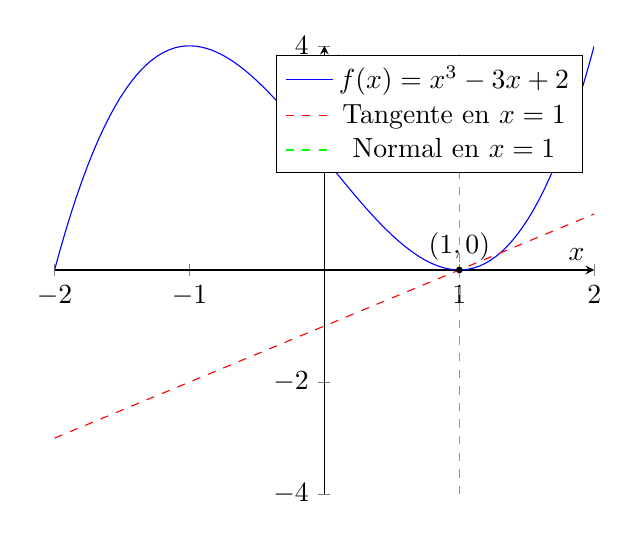
\begin{tikzpicture}
        \begin{axis}[
            axis lines = middle,
            xlabel = $x$,
            ylabel = {$y$},
            xmin = -2, xmax = 2,
            ymin = -4, ymax = 4,
            samples = 100
        ]
        \addplot [
            domain=-2:2, 
            samples=100, 
            color=blue,
        ]
        {x^3 - 3*x + 2};
        \addlegendentry{$f(x) = x^3 - 3x + 2$}
        
        \addplot [
            domain=-2:2, 
            samples=100, 
            color=red,
            dashed
        ]
        {(x - 1)};
        \addlegendentry{Tangente en $x=1$}
        
        \addplot [
            domain=-1:1, 
            samples=100, 
            color=green,
            dashed
        ]
        coordinates {(1,-4)(1,4)};
        \addlegendentry{Normal en $x=1$}
        
        \draw [fill] (axis cs:1,0) circle [radius=1pt];
        \node at (axis cs:1,0) [anchor=south] {$(1, 0)$};
        \end{axis}
    \end{tikzpicture}
\end{center}

\subsection{Derivadas de funciones implícitas}

Las funciones implícitas son aquellas que no están explicitadas en términos de una variable independiente. En lugar de tener una forma \( y = f(x) \), las funciones implícitas están dadas por una ecuación que relaciona \( x \) y \( y \) de forma implícita, como \( F(x, y) = 0 \). Para encontrar la derivada de una función implícita, usamos la técnica de derivación implícita.

\subsubsection{Derivación Implícita}
Para calcular la derivada de una función implícita \( F(x, y) = 0 \), seguimos los siguientes pasos:

Pasos para la Derivación Implícita
\begin{itemize}
    \item \textbf{Diferenciar ambos lados de la ecuación} con respecto a \( x \), tratando \( y \) como una función de \( x \). Esto implica aplicar la regla de la cadena para términos que involucren \( y \)
    \item \textbf{Resolver para \( \frac{dy}{dx} \)}, que es la derivada de \( y \) con respecto a \( x \).
\end{itemize}

\subsection*{Fórmula General}
Dada la ecuación implícita \( F(x, y) = 0 \), la derivada implícita se obtiene de la siguiente manera:
\[
\frac{dF}{dx} = \frac{\partial F}{\partial x} + \frac{\partial F}{\partial y} \cdot \frac{dy}{dx} = 0
\]
\[
\frac{dy}{dx} = -\frac{\frac{\partial F}{\partial x}}{\frac{\partial F}{\partial y}}
\]

\begin{example}
Encuentra la derivada de la función implícita \( x^2 + y^2 = 25 \).

\begin{enumerate}
    \item Diferenciamos ambos lados de la ecuación:
    \[
    \frac{d}{dx}(x^2 + y^2) = \frac{d}{dx}(25)
    \]
    \[
    2x + 2y \frac{dy}{dx} = 0
    \]
    
    \item  Resolviendo para \( \frac{dy}{dx} \):
    \[
    2y \frac{dy}{dx} = -2x
    \]
    \[
    \frac{dy}{dx} = -\frac{x}{y}
    \]
\end{enumerate}
\end{example}

\begin{example}
Encuentra la derivada de la función implícita \( x^3 + y^3 = 6xy \).

\begin{enumerate}
    \item Diferenciamos ambos lados de la ecuación:
    \[
    \frac{d}{dx}(x^3 + y^3) = \frac{d}{dx}(6xy)
    \]
    \[
    3x^2 + 3y^2 \frac{dy}{dx} = 6 \left( x \frac{dy}{dx} + y \right)
    \]
    
    \item  Resolviendo para \( \frac{dy}{dx} \):
    \[
    3x^2 + 3y^2 \frac{dy}{dx} = 6x \frac{dy}{dx} + 6y
    \]
    \[
    3x^2 - 6y = (6x - 3y^2) \frac{dy}{dx}
    \]
    \[
    \frac{dy}{dx} = \frac{3x^2 - 6y}{6x - 3y^2}
    \]
\end{enumerate}
\end{example}


\subsection{Derivadas de orden superior}

Las derivadas de orden superior son derivadas de derivadas. Mientras que la primera derivada de una función proporciona la pendiente de la curva, las derivadas de orden superior brindan información adicional sobre la curvatura y el comportamiento de la función. La segunda derivada, por ejemplo, indica la concavidad de la función, y las derivadas de orden superior se utilizan para análisis más profundos.

\begin{definition}[Derivadas de orden superior]
    Sea \( f(x) \) una función cuya derivada de orden \( n \) existe. La derivada de orden \( n \) de \( f(x) \), denotada como \( f^{(n)}(x) \), se define recursivamente como:
\begin{equation*}
    f^{(1)}(x) = \frac{d}{dx}f(x)
\end{equation*}
\begin{equation}
    f^{(n)}(x) = \frac{d}{dx} f^{(n-1)}(x)
\end{equation}

\end{definition}

\begin{enumerate}
    \item Primera Derivada:
    La primera derivada \( f'(x) \) de una función \( f(x) \) proporciona la pendiente de la tangente en cada punto de la curva.
    \item Segunda Derivada:
    La segunda derivada \( f''(x) \) proporciona información sobre la concavidad de la función. Si \( f''(x) > 0 \), la función es cóncava hacia arriba; si \( f''(x) < 0 \), la función es cóncava hacia abajo.    
    \item Tercera Derivada y Ordenes Superiores:
    Las derivadas de orden superior proporcionan información sobre la tasa de cambio de la concavidad y otros aspectos complejos del comportamiento de la función. Por ejemplo, la tercera derivada \( f'''(x) \) está relacionada con el cambio en la concavidad.
    
\end{enumerate}
\begin{example}
Encuentra la primera, segunda y tercera derivada de la función \( f(x) = x^4 - 3x^3 + 2x - 1 \).
\begin{enumerate}
    \item \textbf{Primera Derivada:}
    \[
    f'(x) = \frac{d}{dx}(x^4 - 3x^3 + 2x - 1) = 4x^3 - 9x^2 + 2
    \]
    
    \item \textbf{Segunda Derivada:}
    \[
    f''(x) = \frac{d}{dx}(4x^3 - 9x^2 + 2) = 12x^2 - 18x
    \]    
    \item \textbf{Tercera Derivada:}
    \[
    f'''(x) = \frac{d}{dx}(12x^2 - 18x) = 24x - 18
    \]
\end{enumerate}
\end{example}

\begin{example}
    Encuentra la primera y segunda derivada de la función \( f(x) = e^x \).

\begin{enumerate}
    \item \textbf{Primera Derivada:}
    \[
    f'(x) = \frac{d}{dx}(e^x) = e^x
    \]
    
    \item \textbf{Segunda Derivada}
    \[
    f''(x) = \frac{d}{dx}(e^x) = e^x
    \]
\end{enumerate}
\end{example}








\section{Aplicaciones de la derivada} % 12 clases
\subsection{Funciones crecientes y decrecientes}

Las derivadas no solo nos informan sobre la pendiente de la curva en un punto, sino que también son fundamentales para determinar el comportamiento global de una función. En particular, la derivada de una función puede indicar dónde la función es creciente o decreciente.

\section*{Definiciones}

\subsection*{Función Creciente}
\begin{definition}[Función Creciente]
    Una función \( f(x) \) es creciente en un intervalo \((a, b)\) si para cualquier par de puntos \( x_1 \) y \( x_2 \) en \((a, b)\) donde \( x_1 < x_2 \), se cumple que:
\[
f(x_1) < f(x_2)
\]
Esto equivale a que su derivada sea positiva en el intervalo:
\[
f'(x) > 0 \text{ para todo } x \text{ en } (a, b)
\]

\end{definition}

\begin{definition}[Función decreciente]
    Una función \( f(x) \) es decreciente en un intervalo \((a, b)\) si para cualquier par de puntos \( x_1 \) y \( x_2 \) en \((a, b)\) donde \( x_1 < x_2 \), se cumple que:
\[
f(x_1) > f(x_2)
\]
Esto equivale a que su derivada sea negativa en el intervalo:
\[
f'(x) < 0 \text{ para todo } x \text{ en } (a, b)
\]
\end{definition}


\begin{example}
Función Polinómica:

Considera la función \( f(x) = x^3 - 3x^2 + 2 \).

\begin{enumerate}
    \item Derivada:
    \[
    f'(x) = \frac{d}{dx}(x^3 - 3x^2 + 2) = 3x^2 - 6x
    \]
    
    \item Encontrar intervalos de crecimiento y decrecimiento:
       \[
       f'(x) = 3x^2 - 6x = 3x(x - 2)
       \]
       La derivada es cero en \( x = 0 \) y \( x = 2 \). Estos puntos dividen la recta en tres intervalos:
       \begin{enumerate}
        \item Para \( x < 0 \): \( f'(x) > 0 \) (función creciente)
        \item Para \( 0 < x < 2 \): \( f'(x) < 0 \) (función decreciente)
        \item Para \( x > 2 \): \( f'(x) > 0 \) (función creciente)
       \end{enumerate}
\end{enumerate}
\end{example}




\begin{example}
Función Exponencial:

Considera la función \( f(x) = e^{-x} \).

\begin{enumerate}
    \item Derivada:
    \[
    f'(x) = \frac{d}{dx}(e^{-x}) = -e^{-x}
    \]
    
    \item Análisis:
       \[
       f'(x) = -e^{-x} < 0 \text{ para todo } x
       \]
       La función es decreciente en todo su dominio.
    
\end{enumerate}
   
\begin{center}
    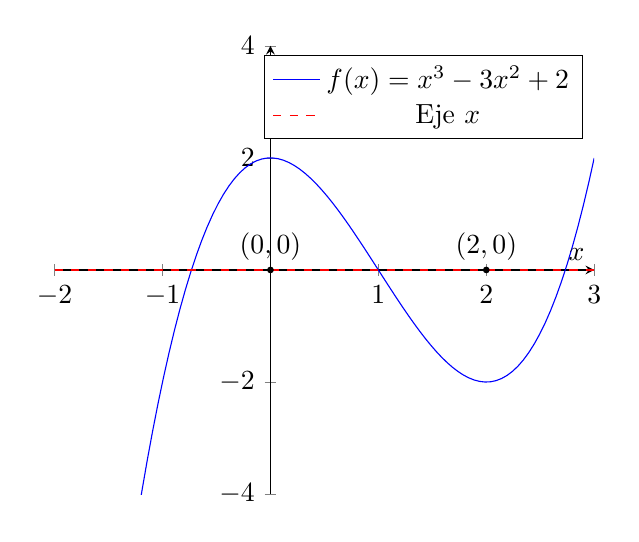
\begin{tikzpicture}
        \begin{axis}[
            axis lines = middle,
            xlabel = $x$,
            ylabel = {$f(x)$},
            xmin = -2, xmax = 3,
            ymin = -4, ymax = 4,
            samples = 100,
            domain = -2:3
        ]
        \addplot [
            domain=-2:3, 
            samples=100, 
            color=blue,
        ]
        {x^3 - 3*x^2 + 2};
        \addlegendentry{$f(x) = x^3 - 3x^2 + 2$}
        
        \addplot [
            domain=-2:3, 
            samples=100, 
            color=red,
            dashed
        ]
        {0};
        \addlegendentry{Eje $x$}
        
        \draw [fill] (axis cs:0,0) circle [radius=1pt];
        \node at (axis cs:0,0) [anchor=south] {$(0, 0)$};
        
        \draw [fill] (axis cs:2,0) circle [radius=1pt];
        \node at (axis cs:2,0) [anchor=south] {$(2, 0)$};
        
        \end{axis}
    \end{tikzpicture}
\end{center}
\end{example}

\subsection{Máximos y mínimos de una función.}

Los máximos y mínimos de una función son puntos críticos que indican los valores más altos y más bajos en un intervalo dado. Estos puntos son fundamentales en el análisis de funciones, especialmente en optimización y en la interpretación gráfica de funciones.

\begin{definition}[Máximo Local]
    Un punto \( x = c \) es un \textbf{máximo local} de una función \( f(x) \) si existe un intervalo abierto alrededor de \( c \) tal que:
\begin{equation}
    f(c) \geq f(x) \text{ para todo } x \text{ en el intervalo}
\end{equation}

\end{definition}
\subsection*{Mínimo Local}

\begin{definition}[Mínimo Local]
    Un punto \( x = c \) es un \textbf{mínimo local} de una función \( f(x) \) si existe un intervalo abierto alrededor de \( c \) tal que:
    \begin{equation}
        f(c) \leq f(x) \text{ para todo } x \text{ en el intervalo}
    \end{equation}
\end{definition}

\begin{definition}[Mázimo y Mínimo Global]
    Un punto \( x = c \) es un \textbf{máximo global} (o absoluto) de \( f(x) \) si:
    \[
    f(c) \geq f(x) \text{ para todo } x \text{ en el dominio de } f
    \]
    
    Un punto \( x = c \) es un \textbf{mínimo global} (o absoluto) de \( f(x) \) si:
    \[
    f(c) \leq f(x) \text{ para todo } x \text{ en el dominio de } f
    \]    
\end{definition}


\subsubsection{Definición de puntos críticos}

Para encontrar los máximos y mínimos de una función \( f(x) \):
\begin{enumerate}
    \item Encuentra la primera derivada \( f'(x) \).
    \item Resuelve \( f'(x) = 0 \) para encontrar los puntos críticos.
    \item Evalúa la segunda derivada \( f''(x) \) en los puntos críticos.
\end{enumerate}

\subsection*{Prueba de la Segunda Derivada}
\begin{enumerate}
    \item Si \( f''(c) > 0 \), \( x = c \) es un mínimo local.
    \item Si \( f''(c) < 0 \), \( x = c \) es un máximo local.
    \item Si \( f''(c) = 0 \), la prueba es inconclusa y puede ser necesario usar otras técnicas.
\end{enumerate}


\begin{example}
    Considera la función \( f(x) = x^3 - 3x^2 + 2 \).
    
    1. Derivadas:
       \[
       f'(x) = 3x^2 - 6x
       \]
       \[
       f''(x) = 6x - 6
       \]
    
    2. Encontrar puntos críticos:
       \[
       3x^2 - 6x = 0 \implies x(x - 2) = 0 \implies x = 0 \text{ o } x = 2
       \]
    
    3. Evaluar la segunda derivada:
       - Para \( x = 0 \):
         \[
         f''(0) = -6 \text{ (máximo local)}
         \]
       - Para \( x = 2 \):
         \[
         f''(2) = 6 \text{ (mínimo local)}
         \]
\end{example}


\begin{example}
Función Exponencial
Considera la función \( f(x) = -x^2 + 4x \).

1. Derivadas:
   \[
   f'(x) = -2x + 4
   \]
   \[
   f''(x) = -2
   \]

2. Encontrar puntos críticos:
   \[
   -2x + 4 = 0 \implies x = 2
   \]

3. Evaluar la segunda derivada:
   Para \( x = 2 \):
     \[
     f''(2) = -2 \text{ (máximo local)}
     \]

\end{example}


\subsubsection{Criterio de la primera derivada para determinar máximos y mínimos}

\begin{enumerate}
    \item Encuentra los Puntos Críticos:
    \begin{enumerate}
        \item Calcula la primera derivada \( f'(x) \).
        \item Resuelve \( f'(x) = 0 \) para encontrar los puntos críticos \( x = c \).
    \end{enumerate}
    \item Analiza el Signo de la Primera Derivada:
    \begin{enumerate}
        \item Para un Máximo Local: Si \( f'(x) \) cambia de positivo a negativo al pasar por \( x = c \), entonces \( x = c \) es un máximo local.
        \item Para un Mínimo Local: Si \( f'(x) \) cambia de negativo a positivo al pasar por \( x = c \), entonces \( x = c \) es un mínimo local.
        \item Punto de Inflexión: Si \( f'(x) \) no cambia de signo alrededor de \( x = c \), el punto \( x = c \) puede ser un punto de inflexión o no tener un comportamiento especial.
    \end{enumerate}
\end{enumerate}


\subsection{Concavidad} 

\subsubsection{Definición de concavidad}
\begin{definition}[Concavidad]
    La \textbf{concavidad} de una función \( f(x) \) describe la forma en que se curva el gráfico de la función. 
\end{definition}
La concavidad se puede clasificar en dos tipos:
\begin{enumerate}
    \item \textbf{Concavidad Hacia Arriba}: Una función es cóncava hacia arriba en un intervalo si su gráfica se curva hacia arriba, como un tazón. En otras palabras, la función tiene una segunda derivada positiva en ese intervalo.
    \item \textbf{Concavidad Hacia Abajo}: Una función es cóncava hacia abajo en un intervalo si su gráfica se curva hacia abajo, como una cúpula. En otras palabras, la función tiene una segunda derivada negativa en ese intervalo.
\end{enumerate}

\subsubsection{Determinación de los Intervalos de Concavidad}
Para determinar los intervalos de concavidad de una función \( f(x) \), sigue estos pasos:
\begin{enumerate}
    \item Calcula la Segunda Derivada:
    Encuentra la segunda derivada \( f''(x) \) de la función.
    \item Encuentra los Puntos Críticos de la Segunda Derivada:
    Resuelve \( f''(x) = 0 \) para encontrar los puntos donde la concavidad podría cambiar. Estos puntos se conocen como puntos de inflexión potenciales. 
    \item Analiza el Signo de la Segunda Derivada:
    \begin{enumerate}
        \item Si \( f''(x) > 0 \) en un intervalo, la función es cóncava hacia arriba en ese intervalo.
        \item  Si \( f''(x) < 0 \) en un intervalo, la función es cóncava hacia abajo en ese intervalo. 
    \end{enumerate}
\end{enumerate}
\subsubsection{Funciones Cóncavas Hacia Arriba y Cóncavas Hacia Abajo}
\begin{itemize}
    \item Función Cóncava Hacia Arriba: Por ejemplo, \( f(x) = x^2 \). La gráfica de esta función es una parábola que se abre hacia arriba.
    \item Función Cóncava Hacia Abajo: Por ejemplo, \( f(x) = -x^2 \). La gráfica de esta función es una parábola que se abre hacia abajo.
\end{itemize}

\subsubsection{Puntos de Inflexión}
\begin{definition}[Puntos de Inflexión]
    Es un punto en la gráfica de una función donde la concavidad cambia de hacia arriba a hacia abajo o viceversa.
\end{definition}
Para identificar un punto de inflexión:
\begin{enumerate}
    \item Encuentra los Puntos Críticos de la Segunda Derivada:
    Resuelve \( f''(x) = 0 \).
    \item Verifica el Cambio de Concavidad:
    Asegúrate de que la concavidad cambia en el punto crítico encontrado.
\end{enumerate}
\subsubsection{Criterio de la Segunda Derivada para la Determinación de Máximos y Mínimos}
El criterio de la segunda derivada se utiliza para clasificar los puntos críticos obtenidos de la primera derivada:

\begin{enumerate}
    \item Encuentra los Puntos Críticos:
    Resuelve \( f'(x) = 0 \) para encontrar los puntos críticos \( x = c \).
 
    \item Calcula la Segunda Derivada en los Puntos Críticos:
    \begin{enumerate}
        \item Si \( f''(c) > 0 \), entonces \( x = c \) es un \textbf{mínimo local}.
        \item Si \( f''(c) < 0 \), entonces \( x = c \) es un \textbf{máximo local}.
        \item Si \( f''(c) = 0 \), el criterio es inconcluso y se debe utilizar otro método para clasificar el punto crítico.
     
    \end{enumerate}
 
\end{enumerate}


\subsection{Análisis de funciones aplicando la derivada.}

El análisis de funciones mediante la derivada permite comprender el comportamiento de las funciones, tales como crecimiento, decrecimiento, y puntos de máximo y mínimo.

\subsection{Problemas de Aplicación}
Los problemas de aplicación de la derivada se dividen en dos categorías principales: problemas de razón de cambio instantáneo y problemas de optimización.

\subsubsection{Problemas de Razón de Cambio Instantáneo}
Estos problemas implican encontrar la tasa de cambio de una función en un punto específico. Para resolver estos problemas:

\begin{enumerate}
    \item Encuentra la derivada de la función.
    \item Evalúa la derivada en el punto de interés para obtener la razón de cambio instantáneo.
\end{enumerate}

\begin{example}
    Considera la función \( f(t) = 2t^3 - 5t^2 + 3 \). Queremos encontrar la razón de cambio instantáneo en \( t = 2 \).

1. Derivada:
   \[
   f'(t) = 6t^2 - 10t
   \]

2. Razón de Cambio Instantáneo en \( t = 2 \):
   \[
   f'(2) = 6(2^2) - 10(2) = 24 - 20 = 4
   \]
   Por lo tanto, la razón de cambio instantáneo en \( t = 2 \) es 4.
   \begin{center}
    \begin{tikzpicture}
        \begin{axis}[
            axis lines = middle,
            xlabel = $t$,
            ylabel = {$f(t)$},
            xmin = 0, xmax = 4,
            ymin = -10, ymax = 20,
            samples = 100
        ]
        \addplot [
            domain=0:4, 
            samples=100, 
            color=blue,
        ]
        {2*x^3 - 5*x^2 + 3};
        \addlegendentry{$f(t) = 2t^3 - 5t^2 + 3$}
        \end{axis}
    \end{tikzpicture}
\end{center}
\end{example}

\subsubsection{Problemas de Optimización}
Los problemas de optimización buscan encontrar los valores máximos o mínimos de una función en un dominio dado. Los pasos para resolver estos problemas son:

\begin{enumerate}
    \item Encuentra la derivada de la función.
    \item Identifica los puntos críticos resolviendo \( f'(x) = 0 \).
    \item Usa la segunda derivada para clasificar los puntos críticos como máximos o mínimos.
    \item Evalúa la función en los puntos críticos y en los límites del dominio para encontrar el valor óptimo.
\end{enumerate}

\begin{example}
    Considera la función \( f(x) = -x^2 + 4x + 1 \). Queremos encontrar el valor máximo de la función.

1. Derivada:
   \[
   f'(x) = -2x + 4
   \]

2. Puntos Críticos:
   \[
   -2x + 4 = 0 \implies x = 2
   \]

3. Segunda Derivada:
   \[
   f''(x) = -2
   \]
   Como \( f''(x) < 0 \), \( x = 2 \) es un máximo local.

4. Valor Máximo:
   \[
   f(2) = -2^2 + 4 \cdot 2 + 1 = -4 + 8 + 1 = 5
   \]
   Por lo tanto, el valor máximo de la función es 5.

   \subsection*{Gráfico para el Problema de Optimización}
   \begin{center}
       \begin{tikzpicture}
           \begin{axis}[
               axis lines = middle,
               xlabel = $x$,
               ylabel = {$f(x)$},
               xmin = 0, xmax = 4,
               ymin = -2, ymax = 10,
               samples = 100
           ]
           \addplot [
               domain=0:4, 
               samples=100, 
               color=red,
           ]
           {-x^2 + 4*x + 1};
           \addlegendentry{$f(x) = -x^2 + 4x + 1$}
           \end{axis}
       \end{tikzpicture}
   \end{center}
   
\end{example}
